\section{1174067 - Kaka Kamaludin}
\subsection{Teori}
\subsubsection{Apa itu generator dengan perumpamaan anda sebagai mahasiswa sebagai generatornya.}
\hfill\break
Generator adalah pembuat dan didalam program, generator adalah pembuat sesuatu. misalnya: 
\begin{figure}[H]
	\centering
	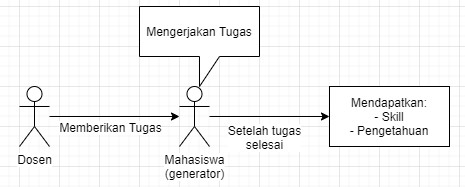
\includegraphics[width=8cm]{figures/1174067/8/1.jpg}
	\caption{Penjelasan no.1}
\end{figure}

\subsubsection{Jelaskan dengan ilustrasi gambar sendiri apa itu diskriminator dengan perumpamaan dosen anda sebagai diskriminatornya.}
\hfill\break
Arti kata diskriminator adalah rangkaian dalam berbagai alat. berasal dari kata diskriminasi yang merujuk pada pelayanan yang tidak adil terhadap individu tertentu, di mana layanan ini dibuat berdasarkan karakteristik yang diwakili oleh individu tersebut. dalam machine learning, Discrimination itu bisa ada dua, yaitu:
\begin{enumerate}
\item Disparate Treatment(perawatan berbeda) atau membedakan/ mengklasifikasikan sesuatu atau seseorang
\item Disparate Impact (dampak berbeda) ialah melihat konsekuensi klasifikasi/ pengambilan keputusan pada kelompok tertentu.
\end{enumerate}
\begin{figure}[H]
	\centering
	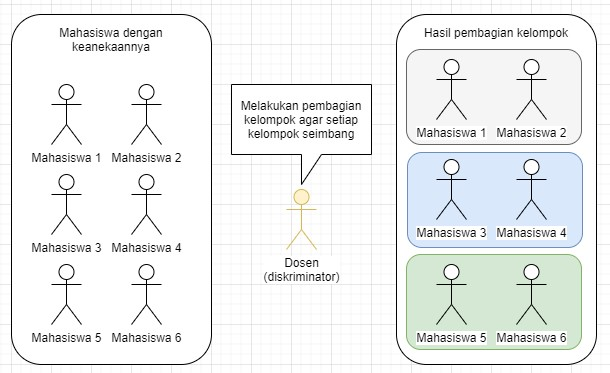
\includegraphics[width=8cm]{figures/1174067/8/2.jpg}
	\caption{Penjelasan no.2}
\end{figure}

\subsubsection{Bagaimana arsitektur generator dibuat}
\hfill\break
Aristektur generator didalam GAN terdiri dari lima lapisan, yaitu: satu input layer, tiga dense layer dan satu output layer.
\begin{figure}[H]
	\centering
	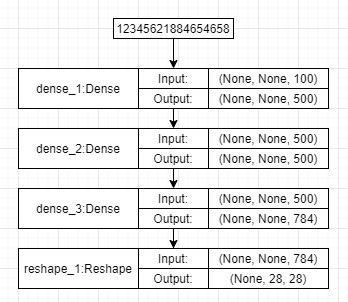
\includegraphics[width=8cm]{figures/1174067/8/3a.jpg}
	\caption{Arsitektur generator pada GAN-Project}
\end{figure}
Dengan ilustrasi sebagai berikut:
\begin{figure}[H]
	\centering
	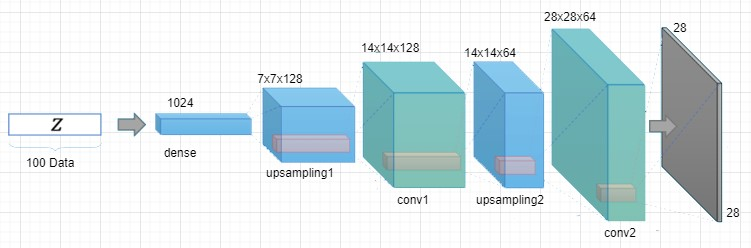
\includegraphics[width=8cm]{figures/1174067/8/3.jpg}
	\caption{Penjelasan no.3}
\end{figure}

\subsubsection{Bagaimana arsitektur diskriminator dibuat}
\hfill\break
aristektur diskriminator didalam GAN terdiri dari lima lapisan, yaitu: satu input layer, tiga dense layer dan satu output layer. Diskriminator pada GAN-Project:
\begin{figure}[H]
	\centering
	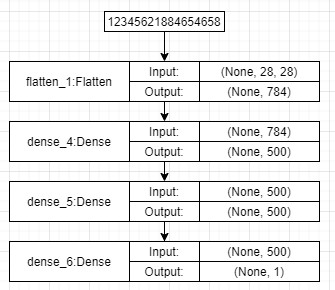
\includegraphics[width=8cm]{figures/1174067/8/4a.jpg}
	\caption{Arsitektur Diskriminator pada GAN-Project}
\end{figure}
Dengan ilustrasi sebagai berikut:
\begin{figure}[H]
	\centering
	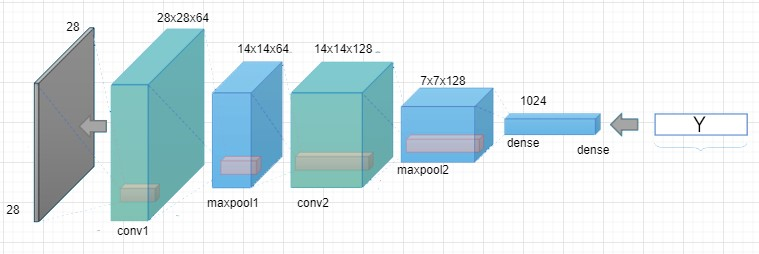
\includegraphics[width=8cm]{figures/1174067/8/4.jpg}
	\caption{Penjelasan no.4}
\end{figure}

\subsubsection{Apa itu latent space.}
\hfill\break
Latent space adalah space atau spot yang tersembunyi, sehingga akan mengambil titik data yang dekat dan yang mirip.
Dengan ilustrasi sebagai berikut:
\begin{figure}[H]
	\centering
	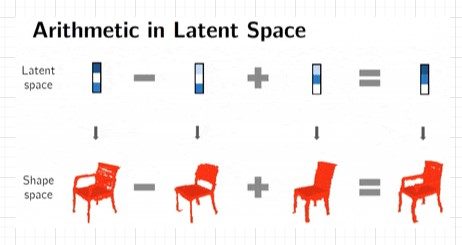
\includegraphics[width=8cm]{figures/1174067/8/5.jpg}
	\caption{Penjelasan no.5}
\end{figure}

\subsubsection{Apa itu adversarial play}
\hfill\break
Dalam GAN adversial play ialah persaingan antara generator dan diskriminator.
\begin{figure}[H]
	\centering
	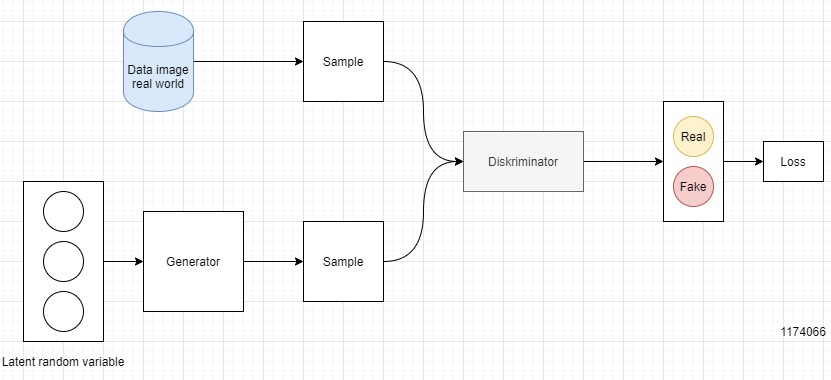
\includegraphics[width=8cm]{figures/1174067/8/6.jpg}
	\caption{Penjelasan no.6}
\end{figure}

\subsubsection{Jelaskan dengan ilustrasi gambar apa itu Nash equilibrium}
\hfill\break
Nash equilibrium adalah strategi yang dipilih oleh masing-masing pemain, dengan strategi pemain lain tertentu.  Strategi ini merupakan strategi terbaik dari masing-masing pemain dengan mempertimbangkan strategi tertentu yang diambil oleh pemain lainnya, atau yang disebut dengan Best Respons.
\begin{figure}[H]
	\centering
	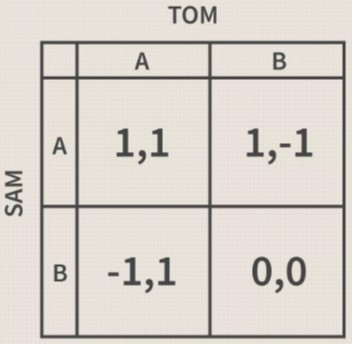
\includegraphics[width=8cm]{figures/1174067/8/7.jpg}
	\caption{Penjelasan no.7}
\end{figure}

\subsubsection{Sebutkan dan jelaskan contoh-contoh implementasi dari GAN}
\hfill\break
Contoh implementasi dari GAN salah satunya adalah men-generate wajah kucing
\begin{figure}[H]
	\centering
	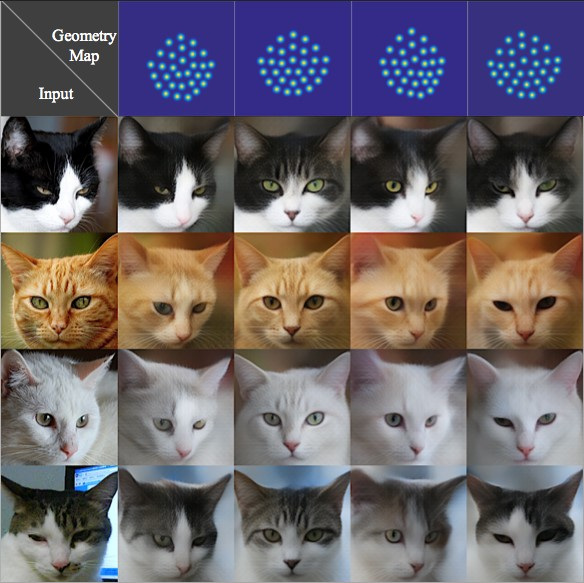
\includegraphics[width=8cm]{figures/1174067/8/8.jpg}
	\caption{Penjelasan no.8}
\end{figure}

\subsubsection{Berikan contoh dengan penjelasan kode program beserta gambar arsitektur untuk membuat generator(neural network) dengan sebuah input layer, tiga hidden layer(dense layer), dan satu output layer(reshape layer)}
\hfill\\
\begin{figure}[H]
	\centering
	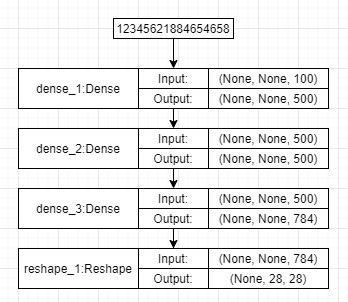
\includegraphics[width=8cm]{figures/1174067/8/3a.jpg}
	\caption{Arsitektur generator pada GAN-Project}
\end{figure}
\lstinputlisting[firstline=10, lastline=22, caption={Kode program arsitektur generator},captionpos=b]{src/1174067/8/1.py}

\subsubsection{Berikan contoh dengan ilustrasi dari arsitektur dikriminator dengan sebuath input layer, 3 buah hidden layer, dan satu output layer.}
\hfill\\
\begin{figure}[H]
	\centering
	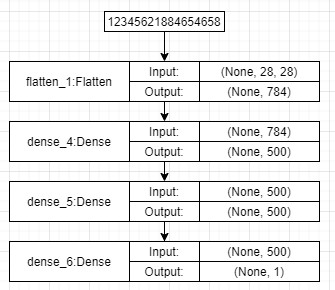
\includegraphics[width=8cm]{figures/1174067/8/4a.jpg}
	\caption{Arsitektur Diskriminator pada GAN-Project}
\end{figure}
\lstinputlisting[firstline=24, lastline=36, caption={Kode program arsitektur diskriminator},captionpos=b]{src/1174067/8/1.py}


\subsubsection{Kaitan output dan input antara generator dan diskriminator tersebut. Jelaskan kenapa inputan dan outputan seperti itu.}
\hfill\break
Kaitan antara output pada generator dan inputan pada diskriminator adalah suatu keterhubungan yang akan menghasilkan data yang benar, karena output dari generator merupakan inoutan pada diskriminator
\begin{figure}[H]
	\centering
	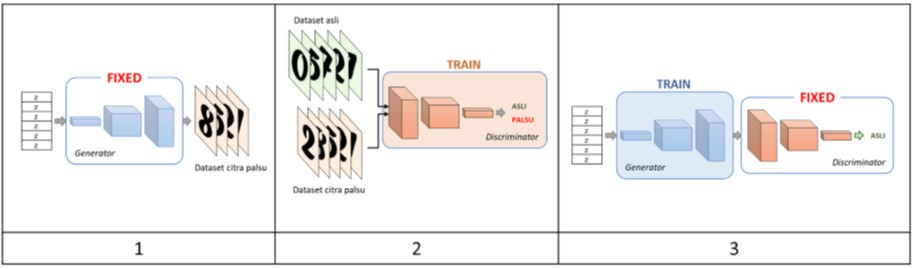
\includegraphics[width=8cm]{figures/1174067/8/9.jpg}
	\caption{Penjelasan no.9}
\end{figure}

\subsubsection{Perbedaan antara Kullback-Leibler divergence (KL divergence)/relative entropy, Jensen-Shannon(JS) divergence / information radius(iRaD) / total divergence to the average dalam mengukur kualitas dari model.}
\hfill\break
diantara keduanya yang paling terkenal adalah KL divergence, karena KL divergence memiliki beberaa sifat/rumus yang bagus .salah satunya adalah KL[q; p] jenis daerah yang di mana q(x) memiliki massa non-null dan p(x) memiliki massa null. Ini mungkin terlihat seperti bug, tetapi sebenarnya ini merupakan fitur dalam situasi tertentu. sedangkan JS tidak memilikinya,

\subsubsection{Fungsi objektif yang berfungsi untuk mengukur kesamaan antara gambar yang dibuat dengan yang asli.} 
\hfill\break
fungsi objektif merupakan fungsi yang akan mengambil parameter data dan model sebagai argumen, dan dapat dievaluasi untuk mengembalikan angka sehingga mampu membedakan gambar yang asli dan yang di buat/fake.

\subsubsection{Scoring algoritma selain mean square error atau cross entropy seperti The Inception Score dan The Frechet Inception distance.} 
\hfill\break
Inception Score digunakan untuk mengukur seberapa realistis output dari GAN, dimana ada dua parameter, yaitu: gambarnya punya variasi dan setiap gambar jelas terlihat seperti sesuatu. Frechet Inception Distance adalah ukuran kesamaan antara dua dataset gambar. Itu terbukti berkorelasi baik dengan penilaian manusia terhadap kualitas visual dan paling sering digunakan untuk mengevaluasi kualitas sampel Generative Adversarial Networks. FID dihitung dengan menghitung jarak Fréchet antara dua Gaussians dipasang ke representasi fitur dari jaringan Inception.

\subsubsection{Kelebihan dan kekurangan GAN} 
\hfill\break
\begin{itemize}
 \item Kelebihan 
   \begin{enumerate}
      \item GAN Menghasilkan data baru yang bisa hampir mirip dengan data asli. Karena hasil pelatihannya, GAN dapat menghasilkan data gambar, teks, audio, dan video yang dapat dibilang hampir mirip dengan yang aslinya. Berkat hal tersebut, GAN dapat digunakan dalam sistem marketing, e-commerce, games,iklan, dan industri lainnya
      \item GAN mempelajari representasi data secara internal sehingga beberapa masalah pada machine learning dapat diatasi dengan mudah
      \item Discriminator yang sudah dilatih dapat menjadi sebuah classifier atau pendeteksi jika data sudah sesuai. Karena Discriminator yang akan menjadi tidak efisien berkat seringnya dilatih
      \item GAN dapat dilatih menggunakan data yang belum dilabeled
   \end{enumerate}
 \item Kekurangan
   \begin{enumerate}  
      \item Data saat diproses oleh metode gan tidak konvergensi
      \item Jenis sampel yang dihasilkan oleh generator terbatas karena modenya terbatas
      \item Ketidak seimbangnya antara generator dan discriminator dapat menyebabkan overfitting atau terlalu dekat dengan hasil sampel
      \item Sangat sensitif dengan data yang sudah diinisiasi sebelumnya
   \end{enumerate}
\end{itemize}


\subsection{Praktek}
\subsubsection{Jelaskan apa itu 3D convolutions}
\hfill\break
3D convolutions adalah operasi konvolusi 3D yang menerapkan filter 3D ke data input dengan tiga arah, yaitu x,y, dan z. fitur ini menciptakan sebuah daftar peta yang ditumpuk. 
\begin{figure}[H]
	\centering
	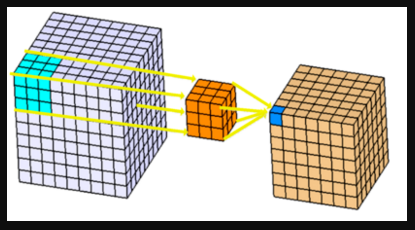
\includegraphics[width=8cm]{figures/1174067/8/no1.png}
	\caption{Penjelasan praktek no.1}
\end{figure}

\subsubsection{Jelaskan dengan kode program arsitektur dari generator networknya, beserta penjelasan input dan output dari generator network.}
\hfill\\
\lstinputlisting[firstline=51, lastline=81]{src/1174067/8/2.py}
Kode di atas akan melakukan create generator ialah gloss, Bentuk jaringan Generator dapat dilihat berkebalikan dengan struktur jaringan saraf pada umumnya. Generator biasanya menerima input sebuah vektor z, yang kemudian mengubahnya menjadi sebuah output 3D atau 3 dimensi.
\begin{figure}[H]
	\centering
	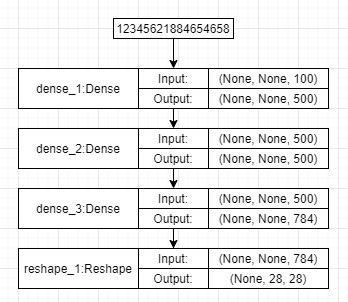
\includegraphics[scale=0.5]{figures/1174067/8/3a.jpg}
	\caption{gambaran proses generator network}
\end{figure}

\subsubsection{Jelaskan dengan kode program arsitektur dari diskriminator network, beserta penjelasan input dan outputnya.}
\hfill\break
\lstinputlisting[firstline=83, lastline=121]{src/1174067/8/2.py}
Diskrimanator adalah d\_loss, Jaringan Discriminator merupakan jaringan klasifikasi biner yang menerima input gambar tiga dimensi dan mengeluarkan klasifikasi menyatakan input gambar adalah gambar asli dari dataset atau merupakan gambar buatan Generator. Diskriminator dilatih dengan dataset yang diambil dari Generator, lalu di training untuk membedakan keduanya. Gambar dari Generator yang berhasil di deteksi oleh Diskriminator sebagai gambar fake, akan dikembalikan dengan feedback pke generator. Kini Generator bertugas untuk bisa membuat sekumpulan gambar palsu, yang nantinya dapat dilihat oleh Diskriminator, lalu, Diskriminator tidak bisa membedakan fake dan real.
\begin{figure}[H]
	\centering
	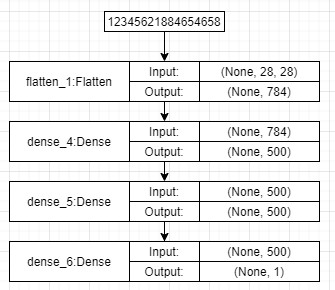
\includegraphics[scale=0.5]{figures/1174067/8/4a.jpg}
	\caption{gambaran proses diskriminator network}
\end{figure}

\subsubsection{Jelaskan proses training 3D-GANs}
\hfill\break
Proses training 3D-GANs dilakukan seperti langkah-langkah berikut:
\begin{itemize}
	\item Terdapat sebuah vektor noise dengan dimensi 200 dari distribusi Gaussian(normal).
	\item Meng-generate gambar palsu menggunakan model generator.
	\item Melatih jaringan generator dengan gambar yang asli(sampel dari data yang real) dan dengan gambar palsu yang dihasilkan oleh generator.
	\item Gunakan adversial model untuk melatih generator model, jangan melatih diskriminator model.
	\item Ulangi langkah ini dengan jumlah epoch tertentu.
\end{itemize}

\subsubsection{Jelaskan bagaimana melakukan settingan awal chapter 02 untuk memenuhi semua kebutuhan sebelum melanjutkan ke tahapan persiapan data.}
\hfill\break
Persiapkan data 3DShapeNets, setelah itu lakukan seperti dibawah ini:
\begin{itemize}
	\item membaca buku panduan dan keterangan dari Generative-Adversial-Network project ini. lalu clone github https://github.com/PacktPublishing/Generative-Adversarial-Networks-Projects
	\item siapkan komputer atau bisa menggunakan google colab
	\item install library sesuai requirements.txt atau membuat virtual env baru dan install librarynya.
\end{itemize}

\subsubsection{Jelaskan tentang dataset yang digunakan, dari mulai tempat unduh, cara membuka dan melihat data. sampai deskripsi dari isi dataset dengan detail penjelasan setiap folder/file yang membuat orang awam paham.}
\hfill\break
Dataset yang digunakan yaitu 3DShapeNets yang berisi model model bentuk benda, folder train berisi model train dan folder test berisi data model testing. dan semua data tersebut di simpan didalam folder volumetric\_data.

\subsubsection{Jelaskan apa itu voxel dengan ilustrasi dan bahasa paling awam}
\hfill\break
Secara singkat, voxel dapat diartikan sebagai 3D pixel atau pixel dalam bentuk 3D
\begin{figure}[H]
	\centering
	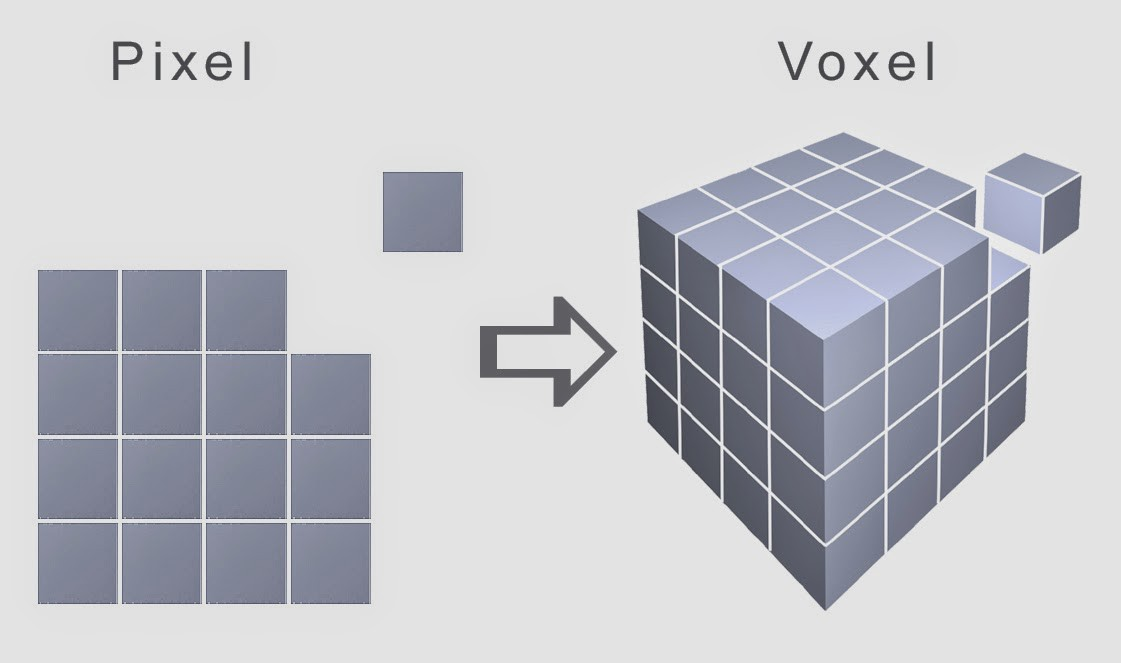
\includegraphics[width=12cm]{figures/1174067/8/no6.png}
	\caption{Gambar Voxel dan Pixel}
\end{figure}

\subsubsection{Visualisasikan dataset tersebut dalam tampilan visual plot, jelaskan cara melakukan visualisasinya}
\lstinputlisting[firstline=11, lastline=28]{src/1174067/8/2.py}
Kode di atas befungsi untuk visualisasidataset dalam tampilan plot. langkah-langkah seperti ini :
	import library, load data file .mat dan lakukan read memakai matplotlib, Hasilnya adalah sebagai berikut:
\begin{figure}[H]
	\centering
	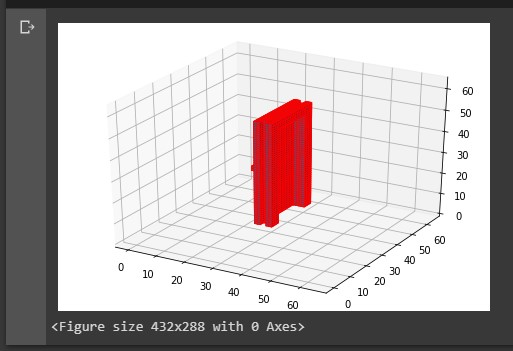
\includegraphics[width=12cm]{figures/1174067/8/no8.jpg}
	\caption{Gambar Voxel dan Pixel}
\end{figure}

\subsubsection{Buka file run.py jelaskan perbaris kode pada fungsi untuk membuat generator yaitu build generator}
\hfill\break
\lstinputlisting[firstline=51, lastline=81]{src/1174067/8/2.py}
Kode di atas befungsi untuk membuat generator yaitu dengan ketentukan gen sebagai variabel dan membuat fungsi atau variabel genmodel lalu dilakukan return. 

\subsubsection{jelaskan juga fungsi untuk membangun diskriminator pada fungsi build discriminator.}
\hfill\break
\lstinputlisting[firstline=83, lastline=121]{src/1174067/8/2.py}
Kode di atas befungsi untuk membangun diskriminator berfungsi untuk mendefenisikan seluruh gambar yang sudah di load generator sebagai gambar fake dan real.

\subsubsection{jelaskan apa maksud dari kode program name == ' main '}
\hfill\break
\lstinputlisting[firstline=171, lastline=171]{src/1174067/8/2.py}
Jika interpreter python menjalankan if name == main sebagai program utama, itu ialah menetapkan variabel name untuk memiliki nilai main. Jika file ini sedang di impor dari modul lain, name akan ditetapkan ke nama modul. Nama modul tersedia sebagai nilai untuk name variabel global.

\subsubsection{jelaskan secara detil perbaris dan per parameter apa arti dari kode program :}
\hfill\break
\lstinputlisting[firstline=172, lastline=185]{src/1174067/8/2.py}
Kode di atas befungsi untuk melakukan load dataset dengan ketentuan data yang hanya dalam folder chair pada data train.

\subsubsection{Jelaskan secara detil dari kode program pembuatan dan kompilasi arsitektur berikut :}
\hfill\break
\lstinputlisting[firstline=187, lastline=198]{src/1174067/8/2.py}
Kode di atas menggunakan Adam sebagai algoritma pengoptimalan dan binary\_crossentropy sebagai kerugian loss. 

\subsubsection{Jelaskan secara detil kode program untuk membuat dan melakukan kompilasi model adversarial berikut:}
\hfill\break
\lstinputlisting[firstline=201, lastline=207]{src/1174067/8/2.py}
Kode di atas artinya ialah kita memasukkan random vector kedalam generator model lalu membagi 2 yaitu generated example dan real example, dan meneruskan ke diskriminator model sebagai real atau fake

\subsubsection{Jelaskan Ekstrak dan load data kursi dengan menggunakan fungsi getVoxelsFormat dan get3DImages yang digunakan pada kode program berikut :}
\hfill\break
\lstinputlisting[firstline=209, lastline=213]{src/1174067/8/2.py}
Kode di atas befungsi untuk melakukan load data pada dataset.

\subsubsection{Jelaskan maksud dari kode program instansiasi TensorBoard yang menambahkan generator dan diskriminator pada program berikut:}
\hfill\break
\lstinputlisting[firstline=215, lastline=218]{src/1174067/8/2.py}
Kode di atas berfungsi untuk membuat tensorboard untuk mencatat log yang akan dihasilkan dari training data kita.

\subsubsection{Jelaskan apa fungsi dari np reshape ones zeros pada kode program berikut dengan parameternya:}
\hfill\break
\lstinputlisting[firstline=220, lastline=222]{src/1174067/8/2.py}
Kode di atas befungsi untuk melakukan reshape agar shape yang dihasilkan tidak terlalu besar. Dengan membuat variabel real dan fake.

\subsubsection{Jelaskan kenapa harus ada perulangan dalam meraih epoch. Dan jelaskan apa itu epoch terkait kode program berikut:}
\hfill\break
\lstinputlisting[firstline=224, lastline=230]{src/1174067/8/2.py}
Kode di atas befungsi untuk melakukan training epoch, karena jika epoch semakin banyak maka kualiatas training yang dihasilkan akan semakin baik dan training epoch akan dilakukan jika variable mode berisikan train.

\subsubsection{Jelaskan apa itu batches dan kaitannya dengan kode program berikut, dan kenapa berada di dalam epoch:}
\hfill\break
\lstinputlisting[firstline=232, lastline=236]{src/1174067/8/2.py}
Batch adalah jumlah file yang akan di training.

\subsubsection{Berikut adalah kode program pengambilan gambar dan noise. Jelaskan apa fungsi np.random.normal serta astype, serta jelaskan apa arti parameter titik dua dan jelaskan isi dari z sample dan volumes batch:}
\hfill\break
\lstinputlisting[firstline=238, lastline=240]{src/1174067/8/2.py}
Kode di atas befungsi untuk gambar menjadi bersih dari noise dan juga menyesuaikan shapenya.

\subsubsection{Berikut adalah kode program generator gambar palsu. Jelaskan apa fungsi generator.predict on batch, serta jelaskan apa arti parameter z sample:}
\hfill\break
\lstinputlisting[firstline=242, lastline=244]{src/1174067/8/2.py}
Kode di atas befungsi untuk membuat sample gambar atau mempredict gambar yang nantinya akan diteruskan ke diskriminator.

\subsubsection{Berikut adalah kode program training diskriminator dengan gambar palsu dari generator dan gambar asil. Jelaskan apa maksudnya harus dilakukan training diskriminator secara demikian dan jelaskan apa isi loss fake dan loss real serta d loss dan fungsi train on batch.}
\hfill\break
\lstinputlisting[firstline=246, lastline=261]{src/1174067/8/2.py}
Kode di atas befungsi untuk membuat diskriminator bisa load gambar fake dan real dari generator, oleh karena itu ada generator loss dan diskriminator loss untuk melihat seberapa baik kualitas yang dihasilkan.

\subsubsection{Berikut adalah kode program training model adversarial yang terdapat generator dan diskriminator. Jelaskan apa bagaimana proses terbentuknya parameter z dan g loss:}
\hfill\break
\lstinputlisting[firstline=262, lastline=271]{src/1174067/8/2.py}
Kode di atas befungsi untuk melakukan print gloss untuk generator dan juga dloss untuk diskriminator.

\subsubsection{Berikut adalah kode program generate dan menyimpan gambar 3D setelah beberapa saat setiap epoch. Jelaskan mengapa ada perulangan dengan parameter tersebut, serta jelaskan arti setiap variabel beserta perlihatkan isinya dan artikan isinya :}
\hfill\break
\lstinputlisting[firstline=273, lastline=282]{src/1174067/8/2.py}
melakukan perulangan dimana setiap terdapat 10 mini-batch akan meng-generate volumenya dan akan menyimpannya lalu membandingkannya.

\subsubsection{Berikut adalah kode program menyimpan average losses setiap epoch. Jelaskan apa itu tensorboard dan setiap parameter yang digunakan pada kode program ini :}
\hfill\break
\lstinputlisting[firstline=284, lastline=287]{src/1174067/8/2.py}
menuliskan log losses ke Tensorboard agar disimpan

\subsubsection{Berikut adalah kode program menyimpan model. Jelaskan apa itu format h5 dan penjelasan dari kode program berikut :}
\hfill\break
\lstinputlisting[firstline=289, lastline=294]{src/1174067/8/2.py}
untuk menyimpan berat model generator dan model diskriminator kedalam file h5.

H5 adalah Hierarchical Data Format 5 File.
File H5 adalah file data yang disimpan dalam Format Data Hirarki (HDF). Ini berisi array multidimensi data ilmiah. File H5 biasanya digunakan di luar angkasa, fisika, teknik, keuangan, penelitian akademis, genomik, astronomi, instrumen elektronik, dan bidang medis.


\subsubsection{Berikut adalah kode program testing model. Jelaskan dengan ilustrasi gambar dari mulai meload hingga membuat gambar 3D dengan menggunakan z sample, bisakah parameter z sample tersebut diubah2? :}
\hfill\break
\lstinputlisting[firstline=296, lastline=314]{src/1174067/8/2.py}
untuk membuat mode predict/prediksi. dimana dia melakukan pebuatan model generator, model diskriminator dan meload data h5 yang sudah dibuat tadi dan meng-generate nya kedalam model 3D, lalu menyimpan model voxel nya ke folder results.
\begin{figure}[H]
\centering
	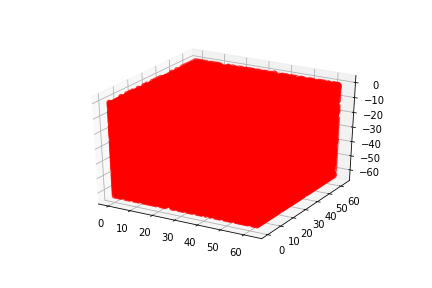
\includegraphics[width=4cm]{figures/1174067/8/img_0_0_0.png}
\caption{Salah satu hasil}
\end{figure}


\subsection{Penanganan Error}
\subsubsection{Error}
\hfill\break
\begin{itemize}
\item OSError

\begin{figure}[H]
\centering
	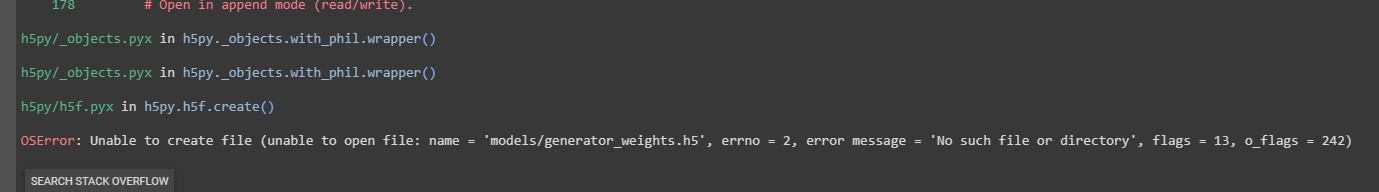
\includegraphics[width=4cm]{figures/1174067/8/error1.jpg}
\caption{OSError}
\end{figure}
\end{itemize}
\subsubsection{Solusi Error}
\hfill\break
\begin{itemize}
\item OSError

Pastikan folder telah ada
\end{itemize}

\subsection{Link Youtube}
https://www.youtube.com/playlist?list=PL4dhp4u89PHbhX9jrGyM3N12gmwhY3uIe